\chapter{Umsetzung}

\section{Aktueller Stand der LSY}
\begin{figure}[h]
	\centering 
	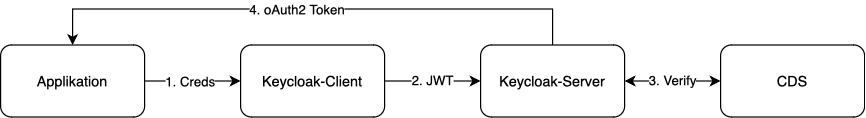
\includegraphics[width=1\textwidth]{img/abbildungen/Unknown.png}
	\captionsetup{format=hang}
	\caption{Aktuelle Umsetzung der Abteilung}
\end{figure}

\begin{itemize}
    \item Innerhalb der Abteilung wird eine passwortbasierte Authentifizierung durchgeführt, welche zusätzlich durch \ac{MFA} geschützt wird.
    \item Webanwendung nutzt einen eigene Anwendung, welche sich als Keycloak-Client aussgibt. Der Nutzer gibt seine Zugangsdaten an den Keycloak-Client weiter, welche diese verarbeitet. Dieser wandelt die Zugangsdaten in einen validen JWT-Token um und übergibt diesen an den Keycloak-Server. Dieser validiert die Zugangsdaten gegen die \ac{CDS}. Ist die Validierung erfolgreich, wird vom Keycloak-Server ein oAuth2-Token erstellt und zurück an die Applikation übergeben.
    \item Innerhalb der \ac{LSY} können sich Applikationen allerdings auch gegen das Azure \ac{AD} authentifizieren lassen. 
\end{itemize}

\section{Integration eines Yubikeys in die LSY}

\begin{figure}[h]
	\centering 
	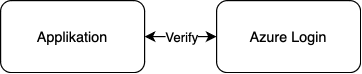
\includegraphics[width=0.6\textwidth]{img/abbildungen/azure_umsetzung.png}
	\captionsetup{format=hang}
	\caption{Umsetzungsmöglichkeit mit Azure \ac{AD}}
\end{figure}

\begin{figure}[h]
	\centering 
	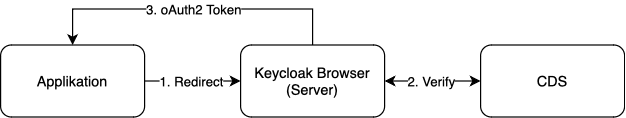
\includegraphics[width=1\textwidth]{img/abbildungen/keycloak_browser.png}
	\captionsetup{format=hang}
	\caption{Umsetzungsmöglichkeit mit Keycloak}
\end{figure}

\begin{itemize}
    \item Grundsätzlich gibt es zwei Möglichkeiten in die aktuelle Applikation eine passwortlose Authentifizierung mit Hilfe eines Yubikeys zu integrieren: Die Nutzung der Authentifizierung gegen das Azure \ac{AD} oder die eine veränderte Nutzung der aktuellen Keycloak-Lösung.
\end{itemize}

\section{User Feedback}
\begin{itemize}
    \item Fragebogen:
    \item How old are you?
    \item What is your role within the team?
    \item Wie zufrieden bist du mit der registrierung? (1-5)
    \item Wie zufrieden bist du mit der Anmeldung? (1-5)
    \item Findest du die passkey variante besser als einen yubikey?
    \item Have you ever used a security key before? Yes, and I still do - Yes, but I stopped using it - No - I don't know
    \item If Yes in which context? (private - work - both)
    \item Do you currently use a password manager at work? (Yes, I use it all/most of the time - Yes, but I only use it sometimes - No)
    \item Do you know how the Fido2 protocol works? (Yes - No - I don't know)
    \item Would you pay for a security key (about 50€)? (Yes - No - I don't know)
    \item Do you think security keys are more secure than passwords? (Yes - No - I don't know)
    \item Comments:
\end{itemize}

\section{Wirtschaftlichkeit}

\section{Nutzung des passwortlosen Verfahrens im privaten Kontext}